\chapter{Method}
\label{chap:method}

\section{Sample fabrication}
\label{sec:sample-fabrication}
A \qty{9}{\mm} by \qty{5}{\mm} undoped \ce{Si} wafer of \qty{500}{\um} thick is used as a substrate. The substrate is spincoated at \qty{2000}{\rpm} with positive resist AR-P 662.06 and baked at \qty{150}{\celsius} for \qty{3}{\min}. This step is then repeated in order to coat 2 layers in total resulting in a total thickness of \qty{1}{\um}. A lithography step is performed using the Raith 100 EBPG exposing the resist to \qty{400}{\micro\coulomb\per\square\cm}. The resist is developed using a 1:3 mixture of MIBK and isopropanol for \qty{45}{\s}, the development is stopped using isopropanol. The Z-407 sputtering machine deposits a \qty{5}{\nm} \ce{MoGe} sticking layer followed by a \qty{500}{\nm} \ce{Au} layer. The lift-off is performed in acetone.

Inside of the inner loop of the coil, we mill a hole of roughly \qty{15}{\um} deep with a diameter of \qty{100}{\um} in the \ce{Si} substrate using a \ce{Ga+} focussed ion beam (Aquilos 2 Cryo-FIB). A similar hole is also made in a microscope coverslip. Using a micromanipulator a \ce{NdFeB} particle of \qty{12}{\um} is placed inside the \ce{Si} hole\footnote{The easiest way to do so is by sticking the particle to the bottom of the needle and then scraping the particle off on the sides of the \ce{Si} hole.} and the coverslip is placed on top of the \ce{Si} substrate. The holes are carefully aligned by moving the coverslip using a micromanipulator. The coverslip is then glued to the \ce{Si} substrate using an epoxy.

The particle is magnetised by putting the whole sample in a magnetic field of approximately \qty{1.3}{\tesla} for several minutes at room temperature and pressure.

A summary of the dimensions of the sample is shown in \autoref{tab:sample-dimensions}. For a schematic illustration of the sample see \autoref{fig:sample-dimensions}.
\begin{SCtable}
    \centering
    \begin{tabular}{lcc}
        \toprule
        \textbf{Parameter} & \textbf{Symbol} & \textbf{Value} \\
        \midrule
        Track thickness & $d$ & \qty{500}{\nm} \\
        Outer track width & $w_1$ & \qty{50}{\um} \\
        Inner track width & $w_2$ & \qty{100}{\um} \\
        Inner loop radius & $r_1$ & \qty{60}{\um} \\
        Outer loop radius & $r_2$ & \qty{120}{\um} \\
        \ce{Si}/Glass hole diameter & & \qty{100}{\um} \\
        \ce{Si}/Glass hole depth & & \qty{15}{\um} \\
        \bottomrule
    \end{tabular}
    \caption{Dimensions of the sample. The radii of the inner and outer loops are their inner radius. Refer to \autoref{fig:sample-dimensions} for further clarification.}
    \label{tab:sample-dimensions}
\end{SCtable}

\begin{figure}
    \centering
    \begin{subfigure}[c]{.5\textwidth}
        \centering
        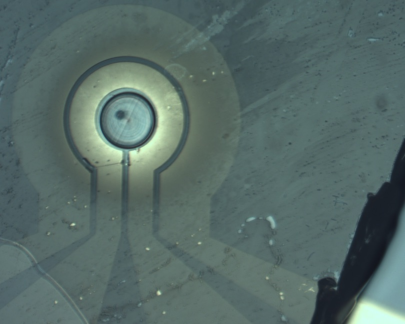
\includegraphics{figures/sample/trap_optical_microscope.pdf}
    \end{subfigure}%
    \begin{subfigure}[c]{.5\textwidth}
        \centering
        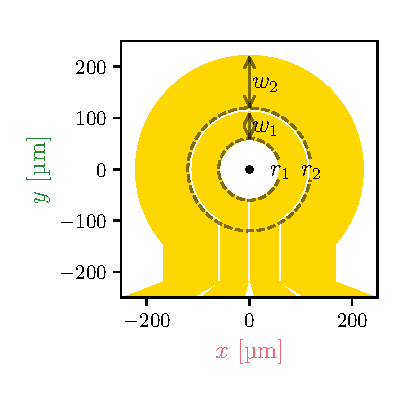
\includegraphics{figures/sample/trap_geometry.pdf}
    \end{subfigure}%
    \caption{An optical microscope image of the sample (\textbf{left}). A couple features can be seen in the image 1) in the bottom left is a discoloration due to the epoxy 2) the dark streak in the bottom right is the edge of the cover glass 3) the dark discoloration is the \ce{Pt} layer of the glass. In the center of the trap you can clearly see the \ce{NdFeB} particle. Furthermore, you can see that their is a small misalignment between the hole in the \ce{Si} and hole in the cover glass. On the \textbf{right} you see a schematic of the sample. A definition of the symbols and their numerical value can be found in \autoref{tab:sample-dimensions}.}
    \label{fig:sample-dimensions}
\end{figure}

\begin{SCfigure}
    \centering
    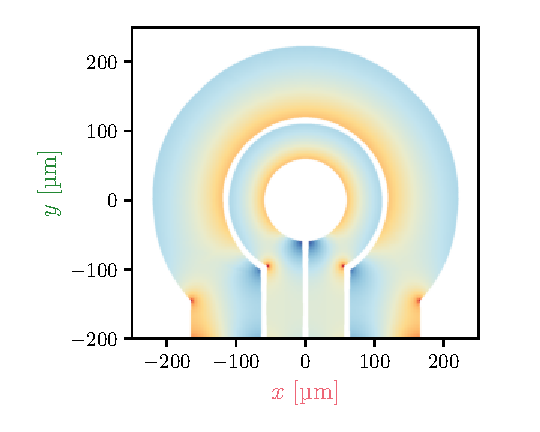
\includegraphics{figures/data/current_through_tracks.pdf}
    \caption{The distribution of current through the tracks. Blue (red) areas indicate a low (high) current density. The simulation was done in COMSOL using a stationary dc-analysis. The current ratio is $\xi = 2$.}
    \label{fig:current-distribution}
\end{SCfigure}

An important design consideration is the distribution of current through the tracks. Simulations in COMSOL show that the current is concentrated in the inside bends. In our case this is beneficial and allows us to get close to the $\xi = 2$ ratio. The current distribution is shown in \autoref{fig:current-distribution}. The extremely high and low currents in the sharp bends are an artefact of the simulation and are not physical.

\section{Experimental setup}
The sample is mounted on a printed circuit board (PCB) with a thick (\qty{1}{\mm}) copper baseplate. The top of the sample is exactly flush with the top of the PCB. Additionally the pads for the wirebonds on the sample and the PCB are aligned and directly next to each other. This allows for very short wirebonds to be used. This significantly reduces the resistance of the wirebonds and thus the maximum current that can be applied to the sample. The wirebonds are made of \qty{25}{\um} thick \ce{Pt}.

The PCB is then placed inbetween two Helmholtz coils with a diameter of \qty{30}{\mm} and 825 windings. They Helmholtz coils provide the uniform magnetic field to align the sample and the gradient magnetic field to control the vertical position of the particle. A dc current on the order of \qty{1}{\ampere} is sent through the coils by two power supplies (Tenma 72-2540).

A microscope objective with a $10\times$ magnification and large working distance is used to provide a visual image of the sample. Additionally a laser (\qty{635}{\nm}, \qty{1}{\milli\watt}) is coupled in. The reflection of the laser is then imaged on a photodiode (ThorLabs PDA36A2). The photodiode is connected to a lock-in amplifier (Zurich Instruments MFLI) allowing for the detection of the motion of the particle. In addition to the photodiode, we can use the camera feed to analyse the motion of the particle. This is done using Python and OpenCV using the CSRT tracker. This tracker is quite robust at the cost of being computationally expensive. As such it cannot be used in real-time.

\section{Simulations}
There are two assumptions in the theory: infinitely thin tracks; and perfectly symmetric loops. Because of this the ideal current ratio will be different in practice. A simulation in COMSOL is used to guide our choice of the current ratio. The simulation is performed in 3D using a stationary dc-analysis.

\subsection{Q-factor}
\label{subsec:q-factor}
In addition to this we estimate our effective Q-factor. A finite Q-factor is caused by damping. Below we discuss several sources of damping.

\subsubsection{Gas damping}
\label{subsubsec:gas-damping}
Gas damping on levitated micrometer sized particles has been studied by \citeauthor{millen}. For pressures above \qty{1E-6}{\milli\bar} and $K_n \ll 1$ stachastic forces dominate the damping rate. The damping rate in this case is given by \autoref{eqn:gas-damping-rate}.

\begin{equation}
    \frac{\Gamma_{\text {gas}}}{2 \pi}=3 \mu_v \frac{a}{m} \frac{0.619}{0.619+K_n} \left( 1+c_K \right)
    \label{eqn:gas-damping-rate}
\end{equation}

$K_n$ is the Knudsen number defined as $K_n = \bar{l}/a$, $\bar{l}$ the mean free path of air molecules, $\mu_v$ the gas viscosity, $a$ the diameter of the particle, $m$ the mass of the particle and the constant $c_K = 0.31 K_n / \left(0.785 + 1.152 K_n + K_n^2 \right)$. A calculation for the gas damping is shown in \autoref{fig:gas-damping}.

\begin{SCfigure}
    \centering
    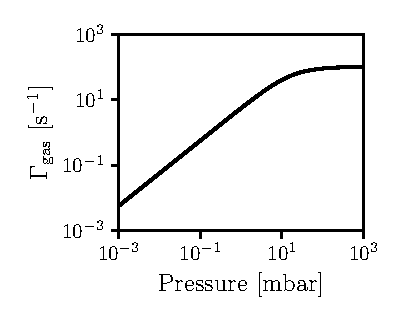
\includegraphics{figures/data/gas_damping.pdf}
    \caption{The gas damping predicted for our particle. The damping rate is calculated using \autoref{eqn:gas-damping-rate}. The calculations have been performed for $T=\qty{300}{\kelvin}$.}
    \label{fig:gas-damping}
\end{SCfigure}

\subsubsection{Inductive damping}
\label{subsubsec:inductive-damping}
The enclosed flux in the loops will change as the particle moves. A changing flux induces a current in the loops which is a dissipative process. Using COMSOL we make an estimate of the dissipation by calculating the induced current in the loops.

TODO: we still need to do this simulation, but I think it will be very similar to the Eddy current damping? Need to check what COMSOL does exactly.

\subsubsection{Eddy current damping}
\label{subsubsec:eddy-current-damping}
Eddy currents are small `whirlpools' of current that are induced by a changing magnetic field. Due to the resistance of the conductor this will lead to dissipation of energy. We consider the case that the moving particle creates a changinging magnetic field which induces the Eddy currents in either the tracks or the residual \ce{Ga} around the trap due to the FIB milling. To estimate the dissipation we perform a simulation in COMSOL where we use the estimated maximum velocity of the particle to include a Lorentz transformation in the magnetic field. The simulation is done in 3D using a stationary dc-analysis.
